\chapter{Energy-based Multi-Modal Attention} 
\label{chapter-emma} 

The literature review (Chapter \ref{chapter-literature-review}) showed that previous research in MMDL has been mostly focused on leveraging the multi-modality to improve the accuracy of the predictions. In this chapter, a new attention module is presented to increase the robustness against failing modes: as long as at least one modality provides enough information for the task, the prediction network will be able to perform well. First, we start by providing a conceptual general framework. Following this, the design of each step of the framework is described. Finally, the training of EMMA is discussed, along with two novel regularizers.

%----------------------------------------------------------------------------------------
%	SECTION 
%----------------------------------------------------------------------------------------

\section{General Framework}\label{sec:general-framework}

We define the i.i.d. dataset $\mathcal{D}^{(N)}$ with $N$ samples  $(\mathbf{X},y)$. The input $\textbf{X}$ is composed of $M$ modes $\{\mathbf{x}_1, \ldots, \mathbf{x}_M\}$ of possibly different dimensions, such as images and sounds. The multi-modal network will be abbreviated as MMN. This model tries to make predictions $\hat{y}$ as close as possible to the groundtruth $y$. The internal architecture of the MMN is often structured as a many-to-one encoder-decoder as discussed in Section \ref{sec:mmdl}. Nonetheless, the EMMA module is not constrained to any specific internal MMN architecture.
\begin{figure}[!h]
\centering
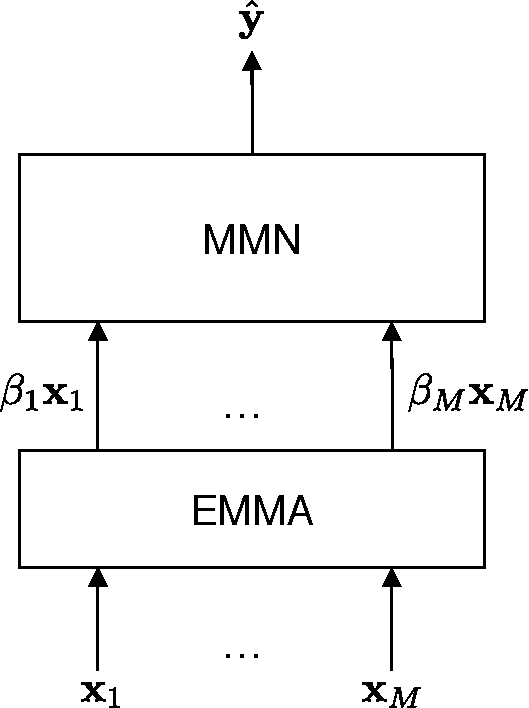
\includegraphics[scale=0.5]{figures/mlp-with-emma}
\caption[High-level view of a Multi-Modal Network with EMMA]{High-level view of a Multi-Modal Network with the EMMA module}	
\label{fig:mnn-with-emma}
\end{figure}

The aim of the attention module is to spontaneously learn to asses how valuable each mode is, on a per-sample basis. The three properties influencing the importance are: relevance, failure intensity and coupling (described in Section \ref{sec:proposed-solution}). To learn this, modal energies are introduced, which are parametric functions embedding the three properties. The modal energy $E_i$ of mode $i$ is of the following form
\begin{equation}
E_i = f(\Psi_i)  + \sum_{k\neq i}^M g[f(\Psi_i), f(\Psi_k)]
\label{eq:general-framework}
\end{equation}
and will have low values if the mode of the sample is important and high values otherwise. The function $f$ is able to capture the relationship between the relevance and the outlyingness (i.e. failure intensity), since $f$ is optimized with respect to the loss on the predictions and is a function of the potential energy. Whereas, the role of the function $g$ is to learn the optimal coupling between modes. Modal energies are then normalized to the importance scores via the Boltzmann distribution, thus going from a measure of absolute importance to one of relative importance. From these importance score, we can determine the attention scores $\beta_i$, representing the quantity of information that can pass through the attention module. Each mode is then multiplied by its respective attention score (see Figure \ref{fig:mnn-with-emma}). It will be made clear later on why the modes are not multiplied by the importance scores instead. Notice that the case of a missing sample in a mode is implicitly solved by definition, if we consider that missing modes are inputs with zeros.

There are two ways of interpreting the proposed solution in this chapter. First, EMMA can be seen as a sort of gate filtering perturbations out. Indeed, failing modes can provoke high activations in the MMN, disturbing the predictions. But by masking the outlying modes we diminish those activations, making it easier for the MMN to make good preditions. Another way to view it, is to understand that the MMN model easily extracts $\beta_i$ and $\mathbf{x}_i$ from the multiplication $\beta_i\mathbf{x}_i$. The model can then learn to make more robust predictions based on the extra inputs $\beta_i$.
\begin{figure}[!ht]
\centering
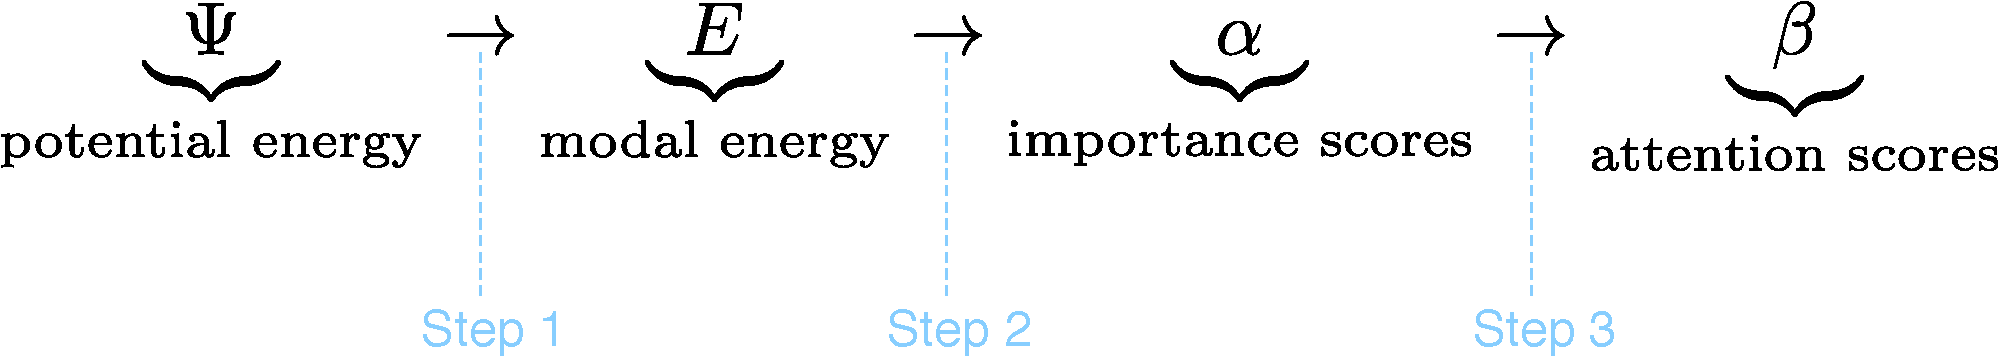
\includegraphics[scale=0.4]{figures/framework}
\caption[Summary of main steps in EMMA]{Summary of main steps in EMMA (step 2, 3 and 4 are detailed in the following sections, step 1 was explained in Chapter \ref{chapter-energy-estimation})}
\end{figure}

%----------------------------------------------------------------------------------------
%	SECTION 
%----------------------------------------------------------------------------------------

\section{From Potential to Modal energies (step 2)}
The \textit{modal energy} of a mode is the sum of its self-energy ($e_i$) and the shared energies ($e_{ij}$) with all the other modes:
\begin{equation}
E_i = e_i + \sum_{k\neq i}^M e_{ij}
\end{equation}

We compute the \textit{self-energy} as a function of the potential energy,
\begin{equation}
e_i = w_i\Psi_i + b_i\,\,\, (=f(\Psi_i)), \qquad w_i, b_i \in \mathbb{R}^+
\label{eq:self-energy}
\end{equation}
where the parameters $w_i$ and $b_i$ are trained via a loss function on the predictions, in consequence the model is able via the self-energy to capture both the relevance and failure. The second advantage of this transformation is that it helps the module to face potentials on different scales, since Equation (\ref{eq:potential-prop}) only guarantees being proportional to the NLL, consequently potentials of different modes may not be on commensurate scales. The reason the parameters are constraint to be positive will be justified below.

Once the self-energies obtained, we can now compute the \textit{shared energies}. The expression $e_{ij}$ denotes the shared energy of mode $j$ on $i$ and is constructed from the self-energies as follows
\begin{equation}
e_{ij} = w_{ij}e_i^{\gamma_{ij}}e_j^{1-\gamma_{ij}}\,\,\, (=g[f(\Psi_i), f(\Psi_j)]), \qquad w_{ij} \in \bigg[-\frac{1}{M-1}, +\frac{1}{M-1}\bigg],\,\, \gamma_{ij} \in [0,1]
\label{eq:shared-energy}
\end{equation}
In an attempt to keep the model interpretable, we add the constraint that $\gamma_{ij} = \gamma_{ji}$. Through the use of shared energies, the model can discover the optimal coupling between the modes. If the model learns a $\gamma_{ij}$ close to zero, mode $i$ and $j$ will influence each other much more than a $\gamma_{ij}$ near to one. In other words, the parameter $\gamma_{ij}$ learns the degree of coupling in the spectrum from strongly coupled ($\gamma_{ij}=0$) to independent ($\gamma_{ij} = 1$). The direction of coupling between mode $i$ and $j$ are learned by the weights $w_{ij}$ and $w_{ji}$. For a positive $w_{ij}$, an increase in self-energy $e_j$ causes an increase in $e_{ij}$, and thus an increase in $e_i$. Whereas if $w_{ij}$ is negative, an increase in $e_j$ leads to a decrease in $e_{ij}$. The weights $w_{ij}$ are not imposed to be equal to $w_{ji}$, such that modes can influence each other asymmetrically. This assymetry is justified by the following example: take a multi-modal problem with three modes A, B and C. We want the model to learn that if mode A is failing, it is optimal that mode B "takes over". And if mode B is failing, it is optimal for C to "take over". This example can only be modelled with asymmetry.

A consequence of the design of Equation (\ref{eq:shared-energy}) is that the evaluation of the gradient during the backpropagation step now involves taking the logarithm of $e_i$\footnote{See Appendix \ref{sec:log-gradient}}, which is undefined for negative values. As the weights in Equation (\ref{eq:self-energy}) are positive, we only have to make sure the values of the potential energy are positive. The latter is done by lowering the potential $\Psi_i$ to Euler's number $\mathrm{e}$ as
\begin{equation}
\Psi_i \leftarrow \max(\mathrm{e}, \Psi_i - \Psi_i^{(\text{min})} + \mathrm{e})
\end{equation}
where $\Psi_i^{(\text{min})}$ denotes the lowest value of $\Psi_i$ in the training set. This correction avoids undefined values ($\Psi_i \geq 0$) but also exploding gradient ($\Psi_i \geq e$). The reason a max-operator is used is because lower energy values than $\Psi_i^{(\text{min})}$  can occur during inference. Of course this correction must be performed prior to the computation of self-energies.

%----------------------------------------------------------------------------------------
%	SECTION 
%----------------------------------------------------------------------------------------

\section{From Modal energies to Importance scores (step 3)}
The importance scores are computed from the modal energies via the Boltzmann distribution:
\begin{equation}
\alpha_i = \frac{1}{Z}e^{-\rho E_i} \quad \text{with the partition function} \quad Z = \sum_{k=1}^M e^{-\rho E_k} 
\label{eq:gibbs-distrib}
\end{equation}
This guarantess the scores to be normalized and summing up to one. A mode $i$ will be said to be important if its score is close to one (low modal energy $E_i$). The hyperparameter $\rho$ represents the coldness, the inverse of the temperature. It controls the entropy of the importance scores distribution. At high temperature ($\rho \rightarrow 0$) the distribution becomes more uniform, and at low temperature ($\rho \rightarrow +\infty$) the importance scores corresponding to the lowest energy tends to 1, while the others approach 0. As can be observed on Figure \,\ref{fig:gibbs}, the coldness has a significant influence on the overall behaviour of the attention module; Careful tuning of $\rho$ is thus necessary.

\begin{figure}[!h]
\centering
\begin{subfigure}{.5\textwidth}
  \centering
  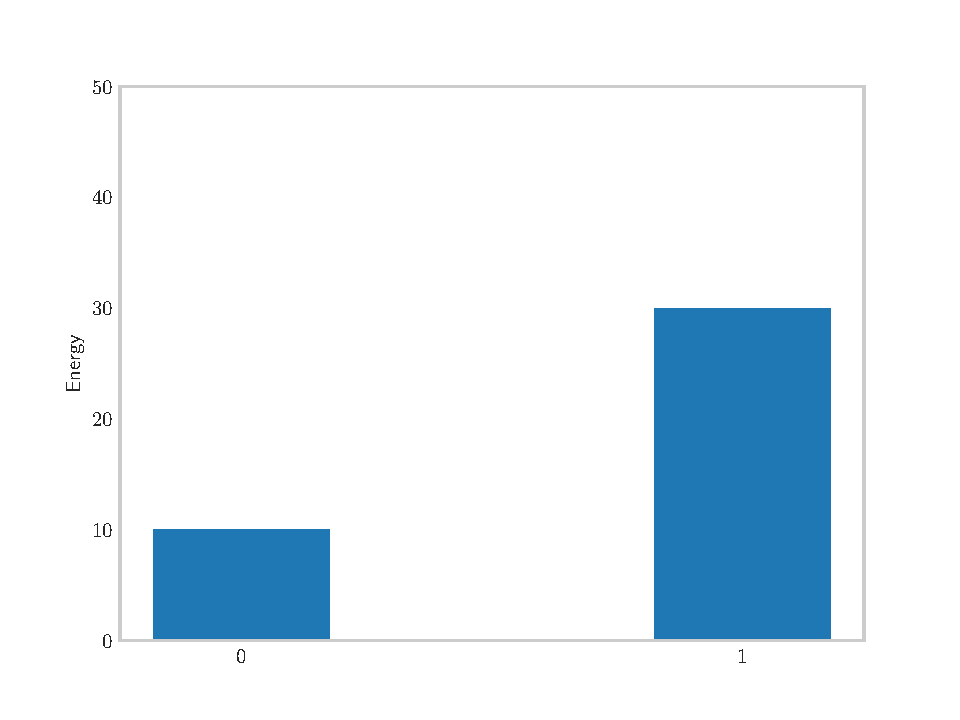
\includegraphics[width=.95\linewidth]{figures/input-gibbs}
  \caption{Energies}
\end{subfigure}%
\begin{subfigure}{.5\textwidth}
  \centering
  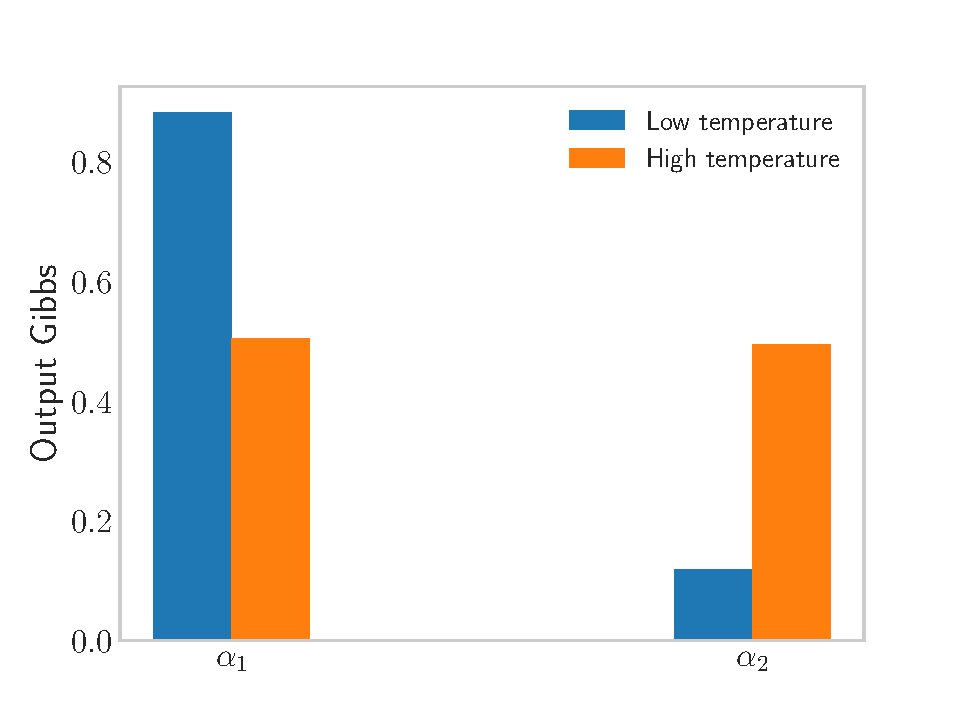
\includegraphics[width=.95\linewidth]{figures/result-gibbs}
  \caption{Importance scores}
\end{subfigure}
\caption[Input-output of Boltzmann distribution for two different temperatures]{Input-output of Boltzmann distribution for two different temperatures, low temperature ($\rho = 0.1$) and high temperature ($\rho = 0.001$)}
\label{fig:gibbs}
\end{figure}


%----------------------------------------------------------------------------------------
%	SECTION 
%----------------------------------------------------------------------------------------

\section{From Importance to Attention scores (step 4)}\label{sec:capacity}
The attention scores are given by
\begin{equation}
\beta_i = \tanh(g_a\alpha_i - b_a) \quad \text{with} \quad g_a > 0,\,\,b_a\in [0,1]
\end{equation}
The hyperbolic tangent adds non-linearity while the gain $g_a$ and bias $b_a$ enable the model to control the threshold and capacity (see Figure \ref{fig:attention-function}). The latter two concepts are detailed below.
\begin{figure}[!h]
\centering
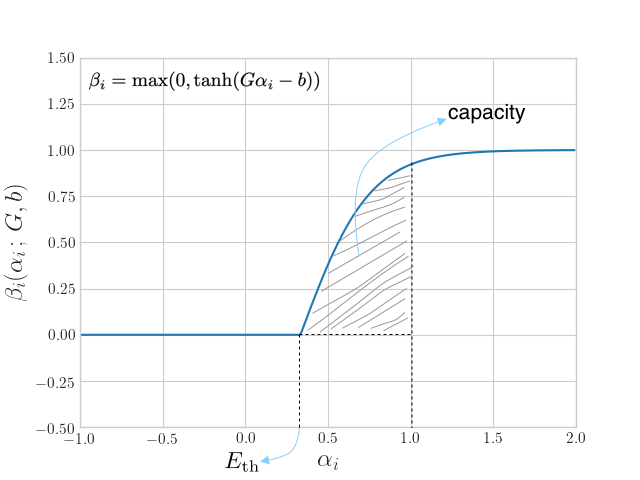
\includegraphics[scale=0.5]{figures/tanh-annotated}
\caption[Attention function]{Attention function (the max-operator generalizes the attention function to cases where $\alpha \in \mathbb{R}$)}
\label{fig:attention-function}
\end{figure}

\subsection*{Energy threshold}
The module will let the information of mode $i$ pass by, only if $g_a\alpha_i - b_a > 0$
\begin{equation}
\begin{split}
&\Leftrightarrow\log(\alpha_i) > \log(b_a/g_a)\\
&\Leftrightarrow E_i \geq \frac{\log(g_a/b_a) - \log(Z)}{\rho} = E_{\text{threshold}}
\end{split}
\end{equation}
where $E_{\text{threshold}}$ represents the maximal amount of energy is allowed to have, to not be completely masked of (see Figure \ref{fig:attention-function}). We deduce that the learned gain and bias control this threshold. Nevertheless, the value of the partition function $Z$ also controls the threshold, making it dynamic. The partition function will be higher if the total energy ($\sum_i E_i$) is higher, resulting in a diminshment of the threshold. To put it in another way, EMMA adapts the selectiveness with respect to the overall quality of the entire input sample. Notice that the influence of the temperature ($\rho^{-1}$) is non-trivial to analyse, because $Z$ also depends on $\rho$.

\subsection*{Capacity}
A more common way to write the attention function would be $\tanh(\mathbf{W}\bm{\alpha}+\mathbf{b})$, whereas we have $\tanh(g_a\mathbf{I}\bm{\alpha}-b_a\mathbf{u})$ with the unit vector $\mathbf{u} = (1 \ldots 1)^T$. We argue the latter better mimics human's attention, permitting us to introduce the concept of capacity, which in psychology is viewed as the amount of resource that can be allocated \citep{attention-is-effort}. If we look at Figure \ref{fig:attention-function}, this can be translated as,
\begin{equation}
\text{capacity} \triangleq \int_0^1 \tanh(g_a\alpha - b_a)d\alpha 
\end{equation}
Define the auxiliary variable $u = g_a\alpha - b_a$. Now using
\begin{equation}
\frac{du}{d\alpha} = g_a \Leftrightarrow d\alpha = \frac{1}{g_a}du
\end{equation}
we can write 
\begin{equation}
\begin{split}
\text{capacity} &= \frac{1}{g_a} \int_0^1 \tanh(u)du  \\
&= \frac{1}{g_a}\log[\cosh(g_a\alpha - b_a)]\bigg\rvert_{\alpha = 0}^1 + \cancel{\text{constant}} \\
&= \frac{1}{g_a}\log\bigg[\frac{\cosh(g_a - b_a)}{\cosh(-b_a)}\bigg]
\end{split}
\end{equation}
When the capacity is too low, no sufficient amount of information is passed to the MMN, leading to wrong predictions. Similarly, if the capacity is too high, the perturbations of the failing modes will pass and cause a decrease in performances. It is expected that the model learns the optimal trade-off, however, if we want the attention module to be robust against failing situations it was not trained on, it can be interesting to try to control this trade-off. To this end, we created a simple regularize which is discussed in the next section. Observe that the concept of capacity can also be applied to $\tanh(\mathbf{W}\bm{\alpha}+\mathbf{b})$, but each mode would have his own capacity, making the importance scores less meaningful.


%----------------------------------------------------------------------------------------
%	SECTION 
%----------------------------------------------------------------------------------------

\section{Training \& Regularization}\label{sec:regul}
The training of the attention module and the prediction model is performed in two stages (see Figure \ref{fig:training}). First, each mode is assigned a separate autoencoder, which is trained on the mode to learn the potential energy function. Once trained, the weights of the autoencoders are freezed. In the second phase, EMMA is inserted in front of the MMN and is trained end-to-end on both normal and corrupted data. By corrupted data, we mean samples on which a corruption process is applied in order to simulate one or more failing modes.

Additionaly, two regularizers are introduced. The first one controls the capacity, where $\lambda_c$ can be positive/negative depending on if we want to maximize/minimize the capacity.
\begin{equation}
\tilde{\mathcal{L}} = \mathcal{L}(y,\hat{y}) + \lambda_c g_a - \lambda_e \Omega \quad \text{with} \quad \Omega = \sum_{k=1}^M \xi_k \log(\alpha_k) \quad \text{and} \quad \xi_k = \begin{cases}
      \xi_- = -1 & \text{if}\ \mathbf{x}_k\, \text{is corrupted} \\
      \xi_+ = +1 & \text{otherwise}
    \end{cases}
\label{eq:regularization}
\end{equation}
Secondly, the purpose of regularizing the energy ($\lambda_e \Omega$) is to control the trade-off between, on one side the relevance and coupling, and on the other side the failure intensity. Without a regularizer, the parameters of the modal energy functions are optimized only regarding the predictions ($\mathcal{L}$), which could lead to a large discrepancy between modal energies $E_i$ and their original potential energies $\Psi_i$. Although the energy regularizer is relatively straightforward, we will show below that some care needs to be taken regarding the corruption process.

\subsection*{Energy regularization}
Let $\bm{\theta}$ be the set of all the parameters in step 2 of the attention module. The effect of the energy regularizer in the SGD algorithm is isolated and written
\begin{equation}
\bm{\theta} \leftarrow \bm{\theta} + \epsilon\lambda_e\nabla_{\bm{\theta}}\Omega
\label{eq:update}
\end{equation}
Remember the objective, we want this update to minimize the discrepancy, thus decrease/increase modal energies $E_i$ for low/high potential energies $\Psi_i$. To verify this let us compute\footnote{the batch is assumed to only contain one sample for the sake of simplicity. However, the demonstration can be generalized to any batch size.} $\nabla_{\bm{\theta}}\Omega$,
\begin{equation}
\nabla_{\bm{\theta}} \Omega =\sum_{k=1}^M \xi_k \nabla_{\bm{\theta}} \log(\alpha_k) 
\label{eq:dev}
\end{equation}
The gradient of the logarithm can be developed as
\begin{equation}
\begin{split}  
\nabla_{\bm{\theta}}  \log(\alpha_k) &= \nabla_{\bm{\theta}} \log \bigg[ \frac{e^{-\rho E_k}}{Z} \bigg] \\
&=  \nabla_{\bm{\theta}}(-\rho E_k) -  \nabla_{\bm{\theta}} \log \sum_{l=1}^M e^{-\rho E_l} \\
&=  -\rho \nabla_{\bm{\theta}}E_k - \frac{\sum_{l=1}^M \nabla_{\bm{\theta}} e^{-\rho E_l}}{\sum_{l=1}^M e^{-\rho E_l}} \\
&= -\rho \nabla_{\bm{\theta}}E_k + \rho \frac{\sum_{l=1}^M e^{-\rho E_l} \nabla_{\bm{\theta}}E_l}{\sum_{l=1}^M e^{-\rho E_l}} \\
&= \rho \Bigg[ -\big(1 - \frac{e^{-\rho E_k}}{Z}\big)\nabla_{\bm{\theta}}E_k + \sum_{l \neq k}^M \frac{e^{-\rho E_l}}{Z} \nabla_{\bm{\theta}}E_l \Bigg] \\
&= \rho \Bigg[ -\big(1 - \alpha_k\big)\nabla_{\bm{\theta}}E_k + \sum_{l \neq k}^M \alpha_l \nabla_{\bm{\theta}}E_l \Bigg] \\
\end{split}
\label{eq:grad-log}
\end{equation}
We go further by expressing the equation above with respect to the subset of parameters $\bm{\theta}_i = \{[\gamma_{ik}, w_{ik}]_{k=1}^M, w_i, b_i\}$:
\begin{equation}
\nabla_{\bm{\theta}_i}  \log(\alpha_k) = \begin{cases}
      -\rho(1-\alpha_i)\nabla_{\bm{\theta}_i}E_i, & \text{if}\, i = k \\
       \rho\alpha_i\nabla_{\bm{\theta}_i}E_i, & \text{if}\, i \neq k
    \end{cases}
\label{eq:log-split}
\end{equation}

The gradient of the regularizer can now be computed by plugging Equation (\ref{eq:log-split}) into the summation (\ref{eq:dev}). Let $M'$ be the number of uncorrupted modes. We obtain for an uncorrupted mode $i$,
\begin{equation}
\nabla_{\bm{\theta}_i}\Omega = \xi_+\big[ -\rho(1-\alpha_i)\nabla_{\bm{\theta}_i}E_i \big] + \big[(M'-1)\xi_+ + (M-M')\xi_-\big]\alpha_i\rho\nabla_{\bm{\theta}_i}E_i
\label{eq:normal-exp}
\end{equation}
and for a corrupted mode $i$,
\begin{equation}
\nabla_{\bm{\theta}_i}\Omega =\xi_-\big[ -\rho(1-\alpha_i)\nabla_{\bm{\theta}_i}E_i \big] + \big[M'\xi_+ + (M-M'-1)\xi_-\big]\alpha_i\rho\nabla_{\bm{\theta}_i}E_i
\label{eq:abnormal-exp}
\end{equation}
Substituting $\xi_k$, we can summarize Equations (\ref{eq:normal-exp}) and (\ref{eq:abnormal-exp}) as
\begin{equation}
\boxed{\nabla_{\bm{\theta}_i}\Omega = -\big[(M-2M')\alpha_i + \xi_i\big]\rho\nabla_{\bm{\theta}_i}E_i}
\end{equation}


Adding the constraint that $M' = \lfloor \frac{M+1}{2} \rfloor$, two cases can be distinguished. If the total number of modes $M$ is even, then we have
\begin{equation}
\bm{\theta}_i \leftarrow \bm{\theta}_i - \epsilon\lambda_e\rho\xi_i\nabla_{\bm{\theta}_i}E_i \quad \text{with} \quad \lambda_e \in \mathbb{R}^+
\end{equation}
Ignoring the second-order effects of the Taylor expansion of the modal energy function, it can be concluded from the equation above that the regularizer will update the parameters such that the values of the modal energy $E_i$ increases/decreases if mode $i$ is corrupted/uncorrupted.

In analogy, if M is uneven we have
\begin{equation}
\bm{\theta}_i \leftarrow \begin{cases}
       \bm{\theta}_i - \epsilon\lambda_e\rho(1-\alpha_i)\nabla_{\bm{\theta}_i}E_i, & \text{if $i$ is uncorrupted} \\
       \bm{\theta}_i + \epsilon\lambda_e\rho(1+\alpha_i)\nabla_{\bm{\theta}_i}E_i & \text{otherwise}
    \end{cases}
\end{equation}
The principle is the same as in the even case with an additional effect: the correction will be proportional to the error. To put it in another way, high energies that must be low and low energies that have to be high will have stronger gradients than their counterparts. This is similar to the positive and negative phase in the optimization of Restricted Boltzmann Machines.

To conclude, let us notice that some undesired effects can appear if we do not add the constraint $M' = \lfloor \frac{M+1}{2} \rfloor$. As an illustration, take $M' = \lfloor \frac{M+1}{2} \rfloor + 1$, Equation (\ref{eq:update}) becomes
\begin{equation}
\bm{\theta}_i \leftarrow \bm{\theta}_i - \epsilon\lambda_e\rho(\alpha_i + \xi_i)\nabla_{\bm{\theta}_i}E_i
\end{equation}
which is unstable for uncorrupted modes leading to a collapse where all energies tend to decrease.

%----------------------------------------------------------------------------------------
%	SECTION 
%----------------------------------------------------------------------------------------

\section{Advantages}
The key advantages of using EMMA are:
\begin{itemize}
\item The generic design of EMMA permits it to be easily added to any type of architecture of a multi-modal model, without modifying nor EMMA nor the MMN.
\item The burden on the MMN is reduced, it only has to learn to make good predictions from the received information. The MMN does not need anymore to learn to distinguish failing modes.
\item The interpretability is increased; It can be verified on a per-sample basis which modes are used to make predictions using the attention scores. As we will see in Chapter 6, EMMA gives us a measure ($\sum_i E_i$) of how uncertain the MMN is about is predictions using the total energy.
\end{itemize}

\newpage
\null
\vfill
\begin{center}
\begin{figure}[!h]
\centering
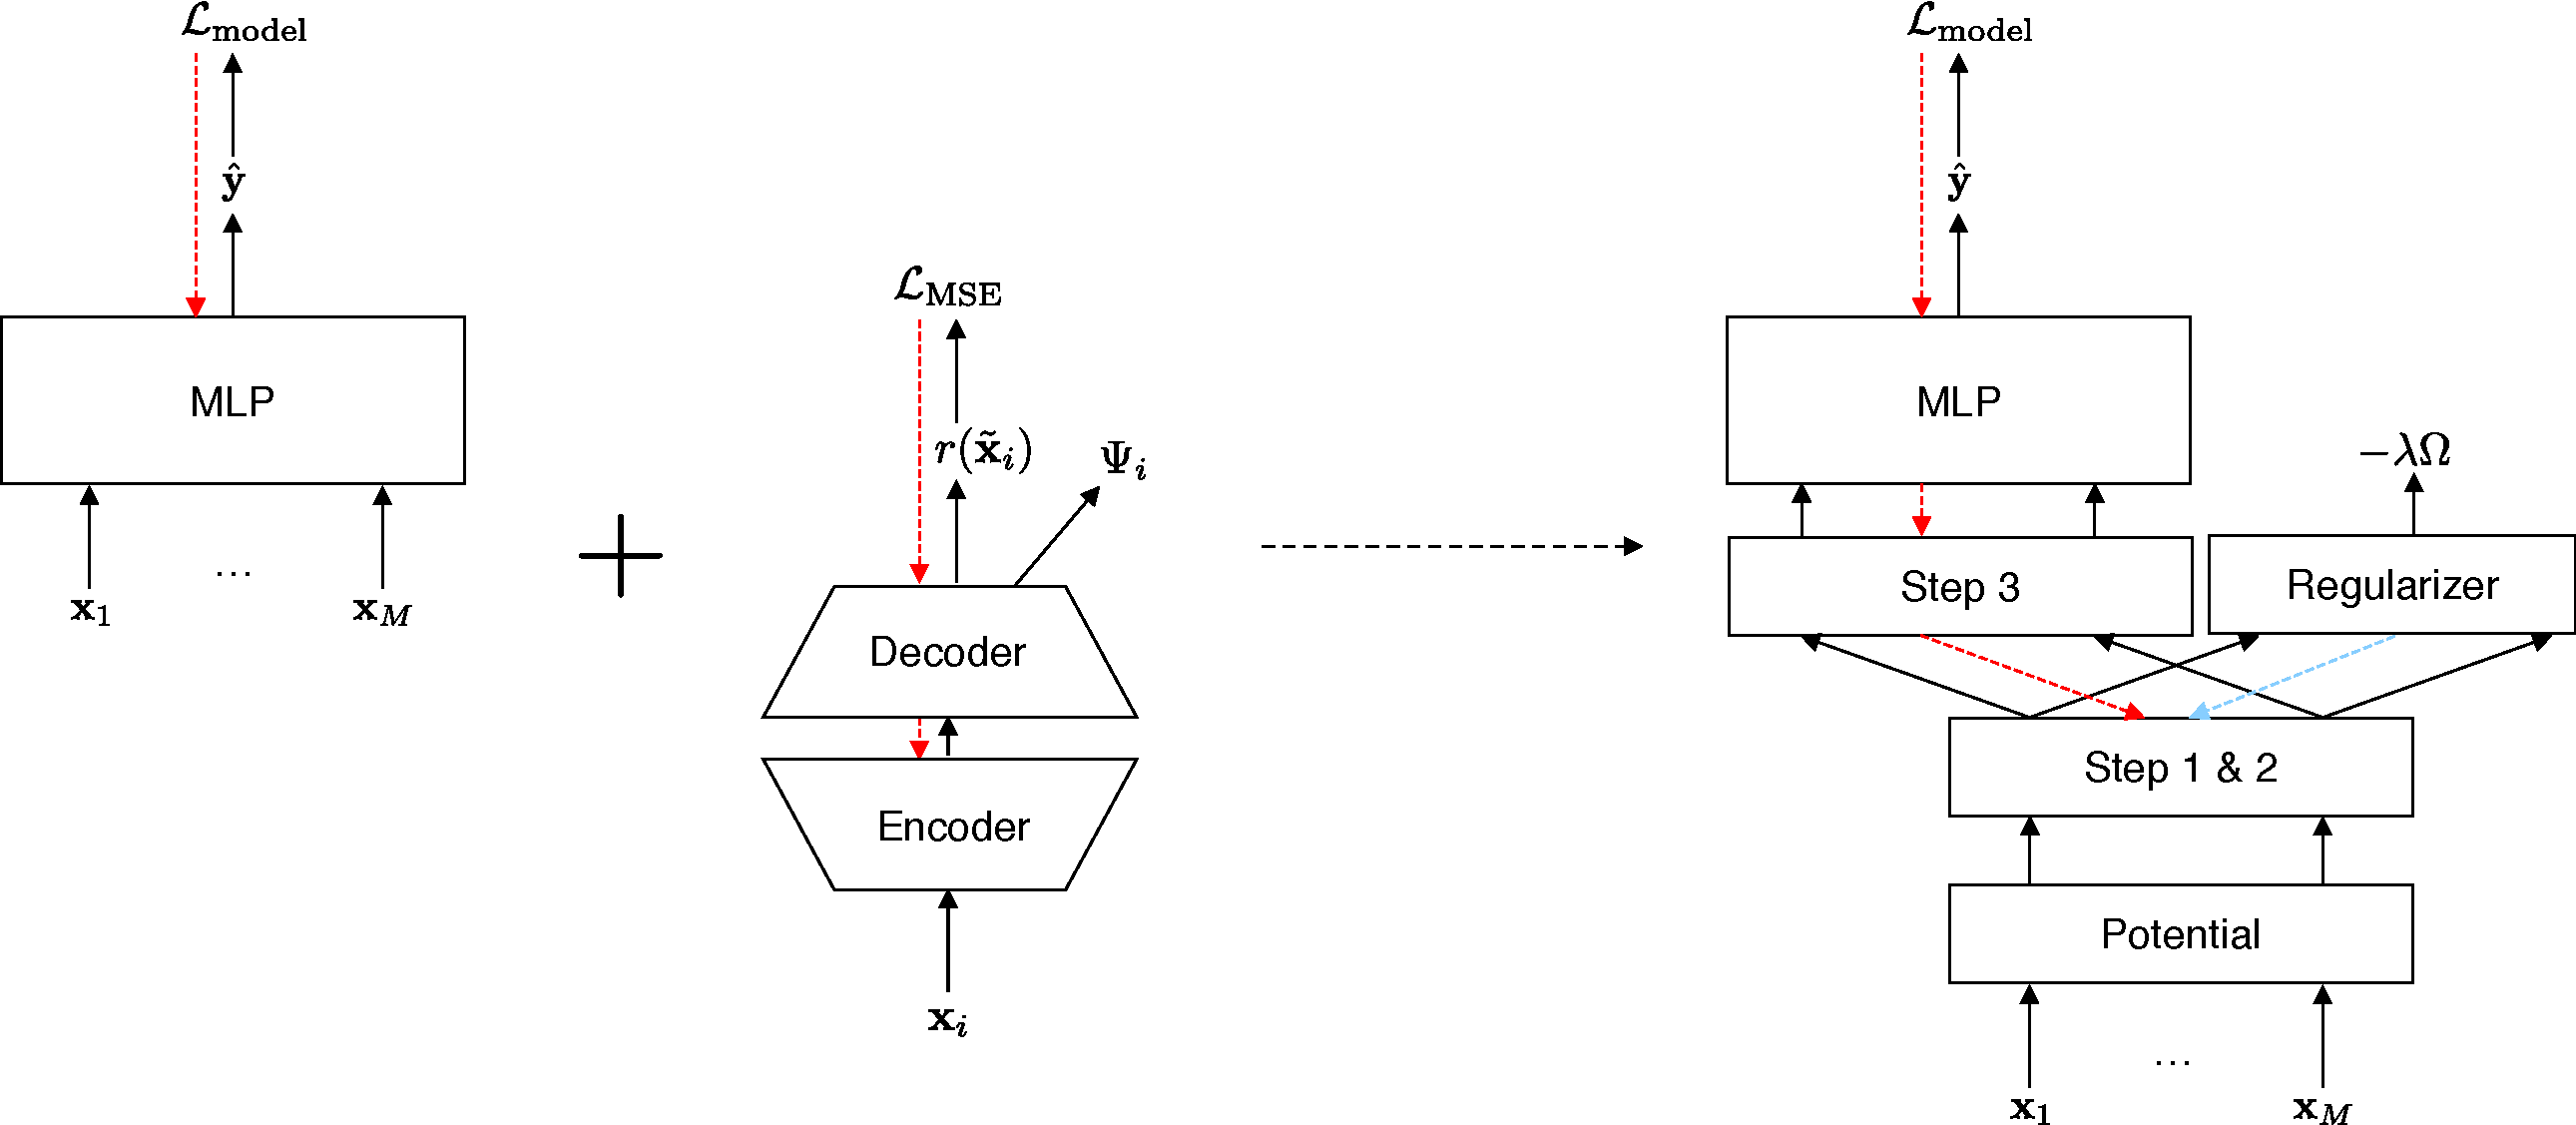
\includegraphics[scale=0.5]{figures/summary-training}
\caption{Summary of end-to-end training}	
\label{fig:training}
\end{figure}
\end{center}
\vfill
\clearpage